\subsubsection{Flöde vid termisk jämvikt}

%To regerenate the figures use /code/pdesolver/generateWallFigApril.m
%with the argument /code/pdesolver/walldata.mat

För att visualisera flödet genom en vägg vid konstant väder och utomhustemperatur görs beräkningar med finita elementmetoden och en konstant inomhustemperatur på $\unit[20]{^\circ C}$. Utomhusvädret är relativ konstant och är satt till antingen molning eller klart och utomhustemperaturen varierar mellan $\unit[6]{^\circ C}$ på natten och $\unit[9]{^\circ C}$ på dagen. Detta har gjorts för en vägg utan och en vägg med isolering, se figur \ref{fig:energyflow_stst}. Den oisolerade väggen består av $\unit[0,5]{m}$ tegel och den isolerade har dessutom $\unit[0,1]{m}$ mineralull. %RESULTAT ur graferna 


\begin{figure}[hpbt]
\centering

\subfloat[Energiflöde ut från insidan av en oisolerad vägg en klar dag.]{
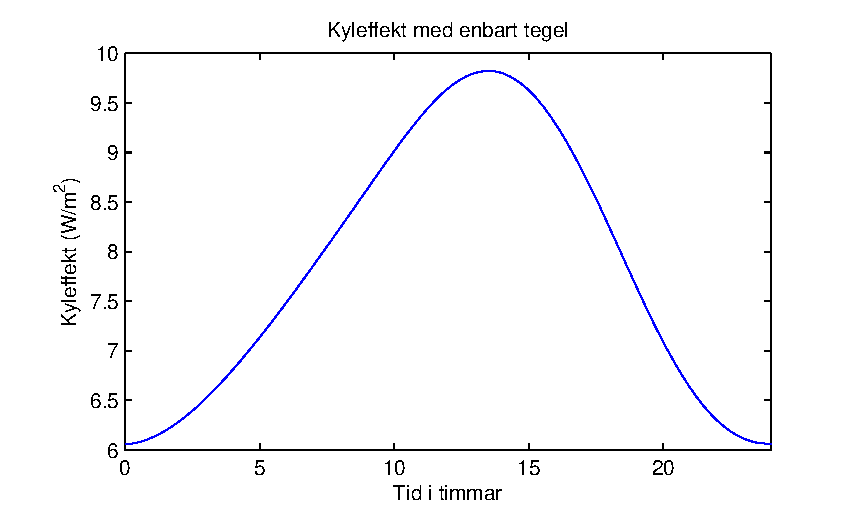
\includegraphics[width=6cm]{images/noinsulationapril.eps}}\vspace{5mm}

\subfloat[Energiflöde ut från insidan av en isolerad vägg en klar dag.]{
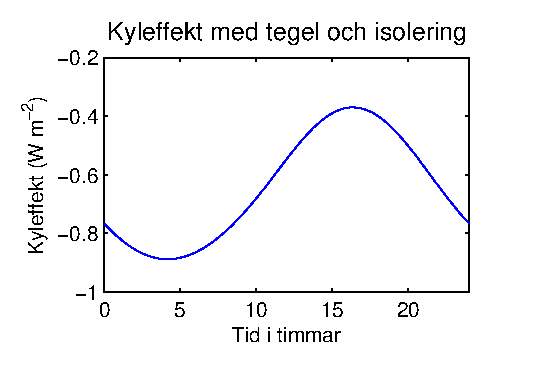
\includegraphics[width=6cm]{images/insulationapril.eps}}

\subfloat[Energiflöde ut från insidan av en oisoleradvägg en molnig dag.]{
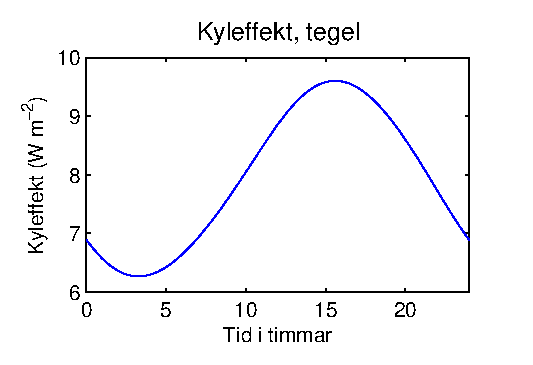
\includegraphics[width=6cm]{images/noinsulationcloud.eps}}\vspace{5mm}

\subfloat[Energiflöde ut från insidan av isolerad vägg en molnig dag.]{
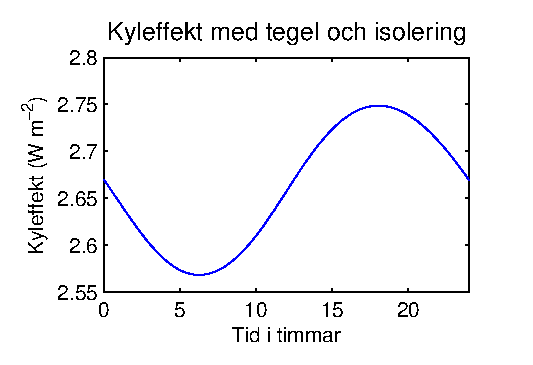
\includegraphics[width=6cm]{images/insulationcloud.eps}
}

\caption{\label{fig:energyflow_stst} Energiflöden ut från insidan av en vägg en dag motsvarande en i mitten av april.
Utomhustemperaturen varierar mellan $\unit[6]{^\circ C}$ på natten och $\unit[9]{^\circ C}$ på dagen. Inomhustemperaturen är satt konstant $\unit[20]{^\circ C}$.}
\end{figure}


Vidare har också energiflödena genom väggen en kall, molnig decemberdag undersökts, alltså en dag där energiflödena bör bli ganska stora. Detta kan ses som ett extremfall på nyår för Göteborg och är då en övre uppskattning på den energiåtgång fastigheten.
 Temperaturen går från $\unit[-5]{^\circ C}$ på dagen till $\unit[-11]{^\circ C}$ Solinstrålningen denna dag är satt till $\unit[20]{\%}$ av vad den skulle varit den den sista december om det varit helt klart. Konvektionskoefficienten har satts till $h=35$ vilket motsvarar en vindhastighet $\unit[5]{m/s}$ parallellt med väggens yta. Beräkningarna är genomförda genom att väggen approximerats med en stav och därefter behandlats med
finita elementmetoden.


\begin{figure}[hpbt]
\centering
\subfloat[Energiflöde en  decemberdag från insidan av en oisolerad vägg en molnig dag]{
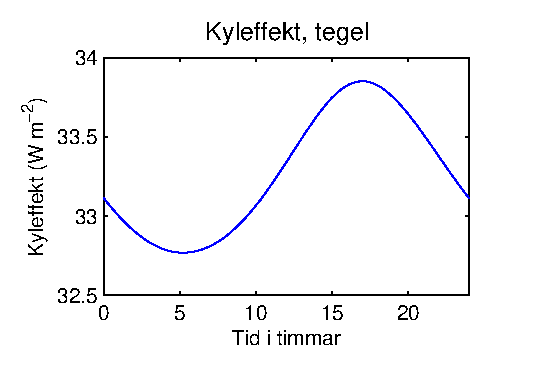
\includegraphics[width=6cm]{images/noinsulationdec.eps}}\vspace{5mm}

\subfloat[Energiflöde från insidan av en isolerad vägg en molnig dag.]{
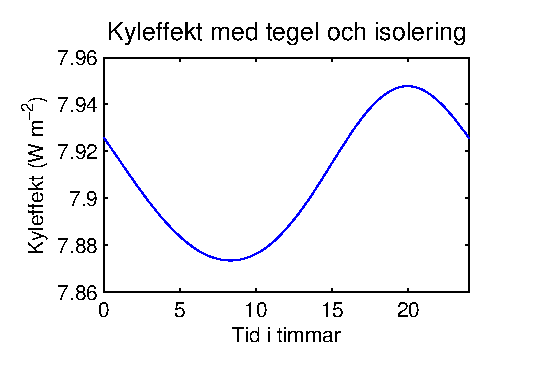
\includegraphics[width=6cm]{images/insulationdec.eps}
}
\caption{Energiflöden ut från insidan av en vägg en dag motsvarande en i december.
}
\end{figure}


Även temperaturfödelningen utanför en vägg har beräknats. Det gjordes med finita element av penaltymetoden. % RESULTAT?
% till diskussion? start
Som kan ses i figur \ref{fig:temp_dist} så existerar anomala temperaturer längs nedre kanten vilket möjligen kan bero på valet av baselement. Ett bättre val skulle kunna vara Streamline-Diffusion/Petrov Galerkin. % till diskussion? slut

\begin{figure}[hpbt]
\centering
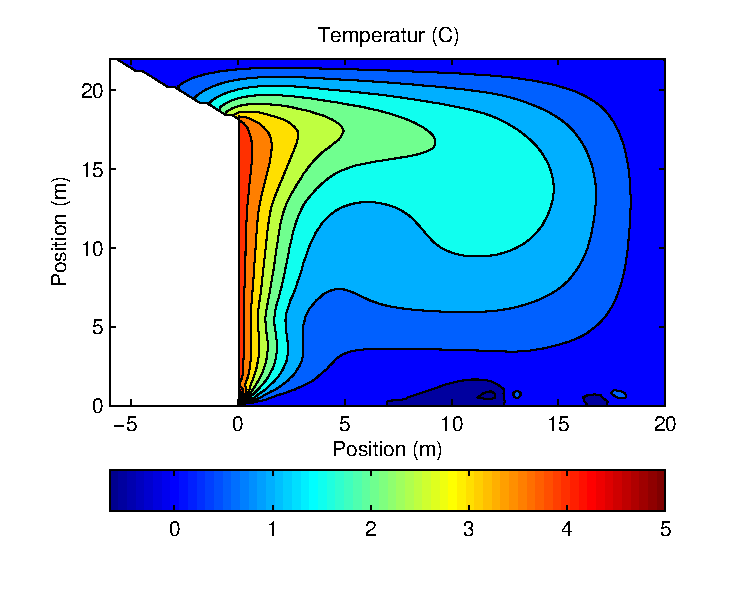
\includegraphics{images/convectemperature.eps}
\caption{\label{fig:temp_dist}Temperaturfördelningen utanför en vägg}
\end{figure}


\textbf{\color{red} Om det inte blir bra resultat så ska det nog inte vara med!} Angående bilderna med hatighetsfältet m.m, \ref{fig:velocityfield}.

\begin{figure}[hpbt]
\centering
\subfloat[Hastighetsfält]{
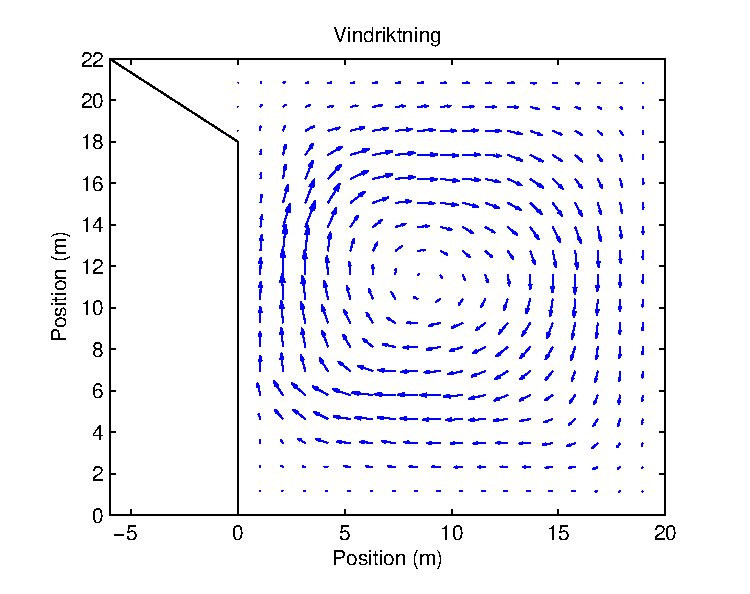
\includegraphics[scale=0.5]{images/convecquiver.eps}
}
\subfloat[Beloppet av hastigheten]{
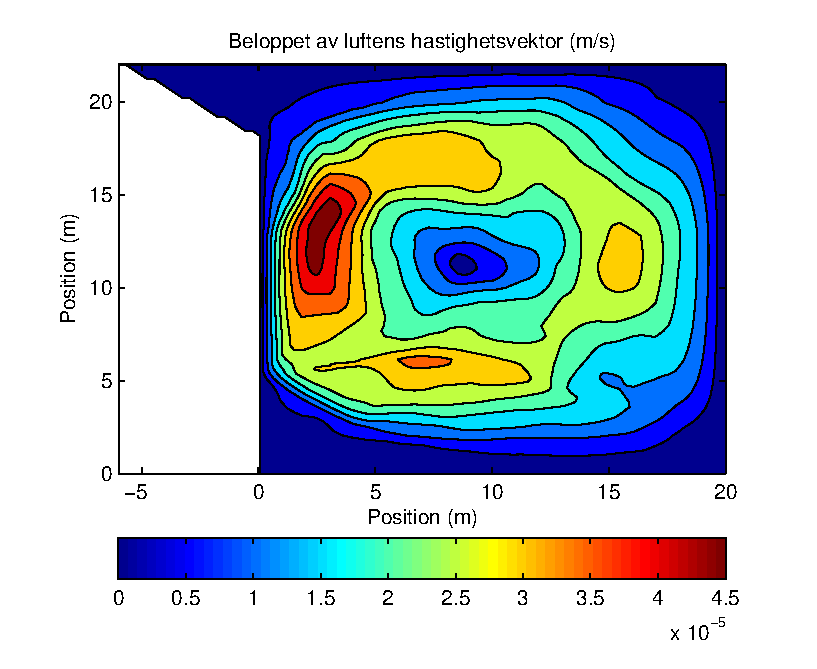
\includegraphics[scale=0.5]{images/convecspeed.eps}
}

\subfloat[Konvektionskoefficienten h mot referenstemperaturen]{
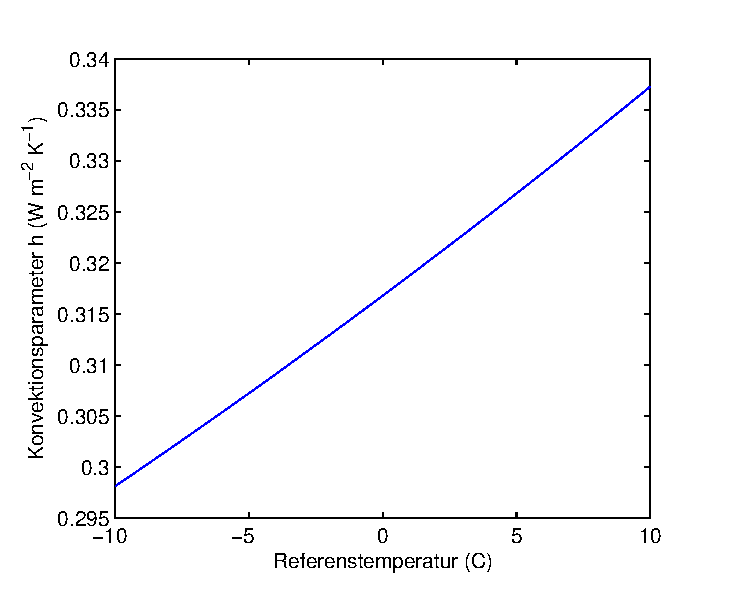
\includegraphics[scale=0.5]{images/convech.eps}
}


\caption{\label{fig:velocityfield}Hastighetsfältet är beräknat med finita element av penalty metoden.

\subfloat[Konvektionskoefficienten h mot penaltyparametern]{
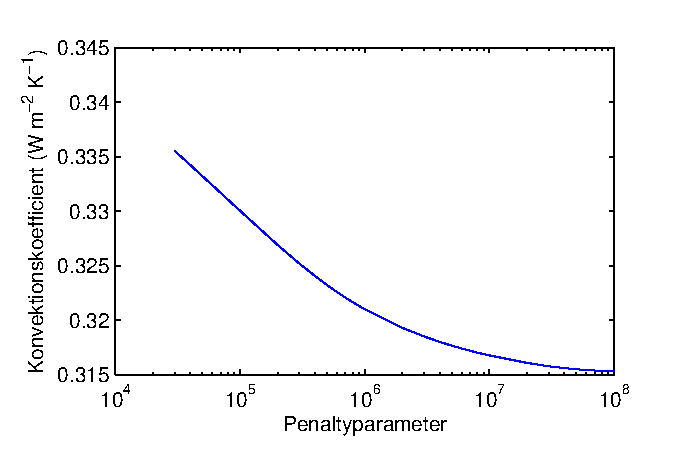
\includegraphics[scale=0.5]{images/convecpenalty.eps}
}\vspace{1cm}
\subfloat[Konvektionskoefficienten h mot den volymetriska expansionskoefficienten.]{
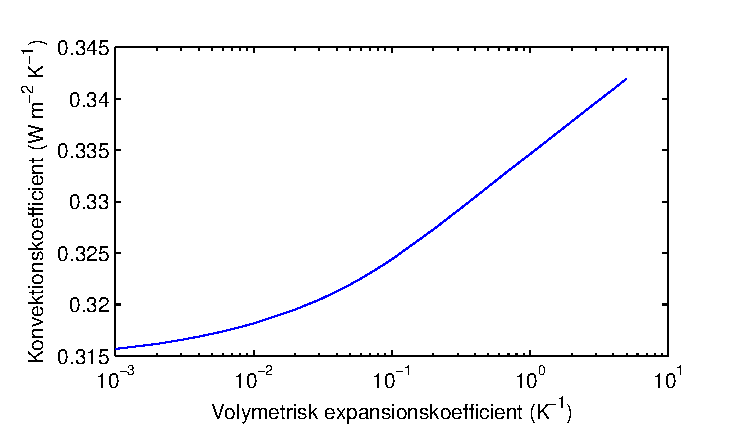
\includegraphics[scale=0.5]{images/convecbeta.eps}
}

\caption{Hastighetsfältet är beräknat med finita element av penalty metoden.
Som kan ses så är hastigheterna orimligt små. Detta medför att konvektionsparametern
blir väldigt liten. Tyvärr verkade det inte som att metodiken som användes för
att framställa ovanstående data fungerade tillräckligt bra för att med någon noggrannhet studera fenomenet konvektion. \emph{\color{red} Dessa bilder måste göras om och deras planering måste funderas igenom.}}

\end{figure}

